% We use \( S \uplus S' \) to denote the disjoint union of sets \( S \) and \( S' \). Let \( \rho = (L \overset{l}{\leftarrowtail} K \overset{r}{\rightarrowtail} R) \) be a rule.
% \newline
% \noindent
%     \begin{minipage}{0.65\textwidth}
%       The DPO diagram for \( G \Rightarrow_\rho H \) with injective match \( m \) can be seen, up to graph renaming, as a diagram in the category of sets where all morphisms are inclusions. The diagram is shown on the right.
%     \end{minipage}
%     \hfill
%     \begin{minipage}{0.34\textwidth}
%           \hfill
%           \resizebox{0.9\textwidth}{!}{
%             \begin{tikzpicture}
%               \coordinate (k) at (0, 0);
%               \draw[fill=white] ($(k)+(0,0)$) rectangle ($(k)+(0.5,0.5)$);
%               \node () at ($(k)+(0.25,0.25)$) {\( K \)};
          
%               \coordinate (c) at (0, -2);
%               \draw[fill=blue!20]
%               ($(c)+(0,-0.5)$)
%               -- ($(c)+(0,0.5)$) 
%               -- ($(c)+(1,0.5)$) 
%               arc[start angle=0, end angle=-90, radius=1]
%               -- cycle;
%               \node () at ($(c)+(0.7,0.2)$) {\( C' \)};
%               \draw[fill=white] ($(c)+(0,0)$) rectangle ($(c)+(0.5,0.5)$);
%               \node () at ($(c)+(0.25,0.25)$) {\( K \)};
          
%               \coordinate (l) at (-3, 0);
%               \draw[fill=orange!20] ($(l)+(-0.5,0)$) rectangle ($(l)+(0.5,1)$);
%               \node () at ($(l)+(-0.2,0.2)$) {\( L' \)};
%               \draw[fill=white] ($(l)+(0,0)$) rectangle ($(l)+(0.5,0.5)$);
%               \node () at ($(l)+(0.25,0.25)$) {\( K \)};
          
%               \coordinate (g) at (-3, -2);
%               \draw[fill=blue!20]
%               ($(g)+(0,-0.5)$)
%               -- ($(g)+(0,0.5)$)
%               -- ($(g)+(1,0.5)$) 
%               arc[start angle=0, end angle=-90, radius=1]
%               -- cycle;
%               \draw[fill=orange!20] ($(g)+(-0.5,0)$) rectangle ($(g)+(0.5,1)$);
%               \node () at ($(g)+(0.7,0.2)$) {\( C' \)};
%               \node () at ($(g)+(-0.2,0.2)$) {\( L' \)};
%               \draw[fill=white] ($(g)+(0,0)$) rectangle ($(g)+(0.5,0.5)$);
%               \node () at ($(g)+(0.25,0.25)$) {\( K \)};
          
%               \coordinate (r) at (3,0);
%               \draw[fill=red!20] ($(r)+(-0.5,0)$)
%                 -- ($(r)+(-0.5,0.5)$)
%                 -- ($(r)+(0,1)$)
%                 --  ($(r)+(0.5,1)$)
%                 -- ($(r)+(0.5,0)$)
%                 -- cycle;
%               \node () at ($(r)+(-0.2,0.2)$) {\( R' \)};
%               \draw[fill=white] ($(r)+(0,0)$) rectangle ($(r)+(0.5,0.5)$);
%               \node () at ($(r)+(0.25,0.25)$) {\( K \)};
          
%               \coordinate (h) at (3, -2);
%               \draw[fill=blue!20]
%               ($(h)+(0,-0.5)$)
%               -- ($(h)+(0,0.5)$)
%               -- ($(h)+(1,0.5)$) 
%               arc[start angle=0, end angle=-90, radius=1]
%               -- cycle;
%               \draw[fill=red!20] ($(h)+(-0.5,0)$)
%               -- ($(h)+(-0.5,0.5)$)
%               -- ($(h)+(0,1)$)
%               --  ($(h)+(0.5,1)$)
%               -- ($(h)+(0.5,0)$)
%               -- cycle;
%              \node () at ($(h)+(0.7,0.2)$) {\( C' \)};
%              \draw[fill=white] ($(h)+(0,0)$) rectangle ($(h)+(0.5,0.5)$);
%              \node () at ($(h)+(0.25,0.25)$) {\( K \)};
%              \node () at ($(h)+(-0.2,0.2)$) {\( R' \)};
          
%               \node (kl) at ($(k)!0.5!(l)+(0.1,0.2)$) {\( \overset{l}{\leftarrowtail} \)}; 
%               \node (kr) at ($(k)!0.5!(r)+(0.1,0.2)$) {\( \overset{r}{\rightarrowtail} \)};  
%               \node (cg) at ($(c)!0.5!(g)+(0.1,0.2)$) {\( \leftarrowtail \)}; 
%               \node (ch) at ($(c)!0.5!(h)+(0.1,0.2)$) {\( \rightarrowtail \)}; 
%               \node (kc) at ($(k)!0.5!(c)+(0.2,0.4)$) {\( \downarrowtail \)}; 
%               \node () at ($(l)!0.5!(g)+(-0.2,0.4)$) {\( m \)}; 
%               \node (lg) at ($(l)!0.5!(g)+(0.1,0.4)$) {\( \downarrowtail \)}; 
%               \node (rh) at ($(r)!0.5!(h)+(0.1,0.4)$) {\( \downarrowtail \)}; 
%             \end{tikzpicture}
%         % \end{center}
%         }
%     \end{minipage}
% \( L', R', C', K \) are mutually disjoint sets such that \( L' \uplus K = L \), \( R' \uplus K = R \), and \( C' \uplus K = C \). 
% Additionally, \( G = L \cup C \) and \( H = R \cup C' \). Thus, any subgraph of \( H \) (resp. \( G \)) can be seen as a union of subgraphs of \( C \) and \( R \) (resp. \( L \)).
% We provide the following definition to improve readability.
% % \begin{definition}
% %         \label{def:corresponding_occurrence}
% %     Let $X$ be a graph and \( G \) a graph. An \textbf{\( X \)-occurrence} in \( G \) is a subgraph of $G$ isomorphic to \( X \). 
% %     Since there is a bijection between \( X \)-occurrences in \( G \) and monomorphisms \( X \rightarrowtail G \), we use the terms \enquote{\( X \)-occurrence} and \enquote{monomorphism from \( X \) to \( G \)} interchangeably.  
% %     An \textbf{implicitly created \( X \)-occurrence} is an \( X \)-occurrence in \( H \) that is included neither in \( R \) nor in \( C \). 
% %     For such an occurrence \( x \), let \( R' = x \cap R \), \( C' = x \cap C \), and let \( h_{R'L}: R' \rightarrowtail L \) be a monomorphism preserving interface elements. The \textbf{corresponding \( X \)-occurrence} relative to \( h_{R'L} \) is \( h_{R'L}(R') \cup C' \).  
% %     An \textbf{implicitly destroyed \( X \)-occurrence} is an \( X \)-occurrence in \( G \) that is not in \( L \) or \( C \).
% % \end{definition}
% \begin{definition}
%         \label{def:subgraph_counting_antipattern:corresponding_occurrence}
%     Let $X$ be a graph and \( G \) a graph. An \textbf{\( X \)-occurrence} in \( G \) is an isomorphism from \( X \) to \( G \).
%     An \textbf{implicitly created \( X \)-occurrence} is an \( X \)-occurrence whose image in \( H \) is included neither in \( R \) nor in \( C \). 
%     For such an occurrence \( x \), let \( R' = x \cap R \), \( C' = x \cap C \), and let \( h_{R'L}: R' \rightarrowtail L \) be a monomorphism preserving interface elements. The \textbf{corresponding \( X \)-occurrence} relative to \( h_{R'L} \) is \( h_{R'L}(R') \cup C' \).  
%     An \textbf{implicitly destroyed \( X \)-occurrence} is an \( X \)-occurrence whose image in \( G \) is neither in \( L \) nor in \( C \).
% \end{definition} 
% Let $X$ be a graph. We define the set \(D(R,X)\) of all subgraphs of \( R \) which can form an implicitly created \( X \)-occurrence with a subgraph of the context graph.
% \begin{definition}[Distinguished subgraphs of the right-hand side graph]
%     \label{def:subgraph_counting_antipattern:rx}
%     % Let \(X\) be a graph and 
%     % \(
%     %     L \overset{l}{\leftarrowtail} K \overset{r}{\rightarrowtail} R
%     % \) an injective DPO rewriting rule.
%     % %  such that $l$ is edge-injective and $r$ is node-injective.
%     % The set \(D(R,X)\) consists of all subgraphs \( R' \subseteq R \) such that there exists a diagram (shown on the right) where
%     % \(h_{R'X} \colon R' \rightarrowtail X \) and \(h_{C'X} \colon C' \rightarrowtail X \) are not isomorphisms, and \(h_{K'K} \colon K' \rightarrowtail K \) and \(h_{R'R} \colon R' \rightarrowtail R \) are inclusion functions. The union of all subgraphs in \( D(R,X) \) is denoted \( R_X \).
%     % Let \(X\) be a graph and 
%     % \(
%     %     L \overset{l}{\leftarrowtail} K \overset{r}{\rightarrowtail} R
%     % \) an injective DPO rewriting rule.
%     % %  such that $l$ is edge-injective and $r$ is node-injective.
%     % The set \(D(R,X)\) consists of all subgraphs \( R' \subseteq R \) such that 
%     % we can construct a diagram as shown on the right where \(h_{K'K} \colon K' \rightarrowtail K \) and \(h_{R'R} \colon R' \rightarrowtail R \) are inclusion functions, and \(h_{R'X} \colon R' \rightarrowtail X \) and \(h_{C'X} \colon C' \rightarrowtail X \) are not isomorphisms. The union of all subgraphs in \( D(R,X) \) is denoted \( R_X \).
%     Let \(\mathcal{X}\) be a ruler-graph with underlying graph \(X\) and
%     \(
%         L \overset{l}{\leftarrowtail} K \overset{r}{\rightarrowtail} R
%     \) an injective DPO rewriting rule.
%     %  such that $l$ is edge-injective and $r$ is node-injective.
%     The set \textbf{\(D(R,X)\)} consists of all subgraphs \( R' \subseteq R \)
%     satisfying the following conditions:
%     \newline
%     \noindent
%     \begin{minipage}{0.7\textwidth}\setlength{\parindent}{1em}
%     \begin{itemize}
%         \item \label{def:drx:rp_not_sub} $R'$ is not a subgraph of $r(K)$,
%         \item \label{def:drx:rp_not_iso} $R'$ is not isomorphic to $X$,
%         \item  \label{def:drx:rp_diagram} a diagram as shown on the right where \(h_{K'K} \colon K' \rightarrowtail K \) and \(h_{R'R} \colon R' \rightarrowtail R \) are inclusion functions can be constructed.
%     \end{itemize}
%     \end{minipage}
%     \todo{condition~\ref{def:drx:rp_diagram} est trop restrictive que la terminaison de [ad hoc protocol, bruggink 2014]}
%     \begin{minipage}{0.299\textwidth}
%         \hfill
%         \resizebox{0.9\textwidth}{!}{
%       \begin{tikzpicture}[node distance=11mm]
%             \node (k) {K};
%             \node (r) [above=of k] {R};
%             \node (r') [right=of r] {$R'$};
%             \node (k') [right=of k] {K'};
%             \node (x)  [right=of r'] {X};
%             \node (c') [below=of x] {C'};
%             \node () [at=($(r)!0.5!(k')$)] {$PB$};
%             \node () [at=($(x)!0.5!(k')$)] {$PO$};
%             \draw[>->] (k) -- (r) node[pos= .5, left] {$r$}; 
%             \draw[>->] (r') -- (r) node[pos= .5, above] {$h_{R'R}$};
%             \draw[>->] (k') -- (k) node[pos= .5, below] {$h_{K'K}$};
%             \draw[>->] (k') -- (r');
%             \draw[>->] (k') -- (c');
%             \draw[>->] (c') -- (x);
%             \draw[>->] (r') -- (x);
%         \end{tikzpicture}
%         }
%     \end{minipage}
%     % The union of all subgraphs in \( D(R,X) \) is denoted \( R_X \).
% \end{definition}  

% The first condition of the definition ensures that any $R' \in D(R,X)$ can be glued along some common interface elements with a subgraph $C'$ of a context graph \( C \) to form an \( X \)-occurrence. The second and third conditions ensure that such $X$-occurrences are included neither in \( C \) nor in \( R \), thereby guaranteeing that they are implicitly created as defined in \autoref{def:corresponding_occurrence}.

% \begin{notation}
% We adopt the visualization conventions from~\cite[Example 9]{overbeek2023apbpotutorial}: labeled graphs are boxed, with their names in the top-left corner; nodes and edges are assigned subsets of \(\mathbb{N}\) as identifiers; identifiers are chosen in such a way that: a node or an edge \( y \) in the codomain graph inherits the union of identifiers from all preimages in the domain, and this assignment uniquely determines the homomorphism. To further improve readability, sets are represented as lists (e.g., \(\{3,4\}\) becomes \(3\ 4\)), and identifiers are omitted when unambiguous. An example is shown below. 
% \begin{center}
%     \resizebox{0.45\textwidth}{!}{
%     \begin{tikzpicture}
%         \graphbox{\( G \)}{00mm}{-20mm}{45mm}{20mm}{2mm}{-5mm}{
%             \coordinate (o) at (-5mm,-8mm); 
%             \node[draw,circle] (l1) at ($(o)+(-10mm,0mm)$) {1};
%             \node[draw,circle] (l2) at ($(l1)+(3,0)$) {2};
%             \node[draw,circle] (l3) at ($(l1)+(1,0)$) {3};
%             \node[draw,circle] (l4) at ($(l1)+(2,0)$) {4};
%             \draw[->] (l1) -- (l3) node[midway,above] {$a$};
%             \draw[->] (l3) -- (l4) node[midway,above] {$b$};
%             \draw[->] (l4) -- (l2) node[midway,above] {$a$};
%         }  
%         \graphbox{\( H \)}{50mm}{-20mm}{34mm}{20mm}{2mm}{-5mm}{
%             \coordinate (o) at (0mm,-8mm); 
%             \node[draw,circle] (l1) at ($(o)+(-10mm,0mm)$) {1};
%             \node[draw,circle] (l2) at ($(l1)+(2,0)$) {2};
%             \node[draw,circle] (l3) at ($(l1)+(1,0)$) {3\ 4};
%             \draw[->] (l1) -- (l3) node[midway,above] {$a$};
%             \draw[->] (l3) edge[loop above] (l3) node[midway,above] {$b$};
%             \draw[->] (l3) -- (l2) node[midway,above] {$a$};
%         }      
%         % \node () at (53mm,-30mm) {$\rightarrow$};
%     \end{tikzpicture}
%     }
% \end{center}  
% \end{notation}


% \begin{example}
%     \label{ex:grsaa_rx}
%     Consider the injective DPO rule from \cite[Example 6]{bruggink2014termination}:  
%     \begin{center} 
%         \resizebox{0.7\textwidth}{!}{
%         \begin{tikzpicture}
%             \graphbox{$L$}{0mm}{0mm}{34mm}{15mm}{2mm}{-5mm}{
%                 \coordinate (o) at (0mm,-3mm); 
%                 \node[draw,circle] (l1) at ($(o)+(-10mm,0mm)$) {1};
%                 \node[draw,circle] (l2) at ($(l1)+(2,0)$) {2};
%                 \node[draw,circle] (l3) at ($(l1) + (1,0)$) {3};
%                 \draw[->] (l1) -- (l3) node[midway,above] {$a$};
%                 \draw[->] (l3) -- (l2) node[midway,above] {$a$};
%             }     
%             \graphbox{$K$}{40mm}{0mm}{24mm}{15mm}{2mm}{-5mm}{
%                 \coordinate (o) at (5mm,-3mm); 
%                 \node[draw,circle] (l1) at ($(o)+(-10mm,0mm)$) {1};
%                 \node[draw,circle] (l2) at ($(l1)+(1,0)$) {2};
%                 % \node[draw,circle] (l3) at ($(l1) + (1,0)$) {$\ $};
%                 % \draw[->] (l1) -- (l3) node[midway,above] {$a$};
%                 % \draw[->] (l3) -- (l2) node[midway,above] {$a$};
%             }    
%             \graphbox{$R$}{70mm}{0mm}{45mm}{15mm}{2mm}{-5mm}{
%                 \coordinate (o) at (-5mm,-3mm); 
%                 \node[draw,circle] (l1) at ($(o)+(-10mm,0mm)$) {1};
%                 \node[draw,circle] (l2) at ($(l1)+(3,0)$) {2};
%                 \node[draw,circle] (l3) at ($(l1) + (1,0)$) {4};
%                 \node[draw,circle] (l4) at ($(l1) + (2,0)$) {5};
%                 \draw[->] (l1) -- (l3) node[midway,above] {$a$};
%                 \draw[->] (l3) -- (l4) node[midway,above] {$b$};
%                 \draw[->] (l4) -- (l2) node[midway,above] {$a$};
%             }    

%             \node () at (37mm,-8mm) {$\leftarrowtail$};
%             \node () at (67mm,-8mm) {$\rightarrowtail$};

%             % \draw[>->] (51mm,2mm) -- (52mm,3mm);
%         \end{tikzpicture}
%         }
%     \end{center}
%     Let $X$ be \tikz[baseline=-0.5ex]{
%         \node (x) at (0,0) {$\bullet$};
%         \node (y) at (1,0) {$\bullet$ };
%         \node (z) at (2,0) { $\bullet$};
%         \draw[->] (x) -- (y) node[midway, above] {$a$};
%         \draw[->] (y) -- (z) node[midway, above] {$a$};
%     } and $R' \in D(R,X)$. 
%     $R'$ is neither the empty graph nor isomorphic to $X$, by Conditions 2 and 3 of \autoref{def:rx}. 
%     Therefore, $R'$ must contain an interface node (either node 1 or node 2), because if it contains no interface node, Condition 1 of \autoref{def:rx} would be violated due to $X$'s connectivity.
%     Additionally, $R'$ must contain node 4 or node 5 to avoid being a subgraph of $r(K)$ (Condition 2). 
%     Therefore, $R'$ must contain either $1 \overset{a}{\to} 4$ or $5 \overset{a}{\to} 2$, because if node 4 or node 5 is isolated, Condition 1 would be violated due to $X$'s connectivity.
%     Furthermore, $R'$ must not contain $4 \overset{b}{\to} 5$ by Condition 1.
%     The following graph is not in $D(R,X)$ because it violates Condition 1.
%    \begin{center}
%         \resizebox{0.24\textwidth}{!}{
%             \begin{tikzpicture}
%                 \graphbox{}{70mm}{0mm}{45mm}{15mm}{2mm}{-5mm}{
%                     \coordinate (o) at (-5mm,-3mm); 
%                     \node[draw,circle] (l1) at ($(o)+(-10mm,0mm)$) {1};
%                     \node[draw,circle] (l3) at ($(l1) + (1,0)$) {4};
%                     \node[draw,circle] (l2) at ($(l1)+(3,0)$) {2};
%                     \node[draw,circle] (l4) at ($(l1) + (2,0)$) {5};
%                     \draw[->] (l4) -- (l2) node[midway,above] {$a$};
%                     \draw[->] (l1) -- (l3) node[midway,above] {$a$};
%                 }    
%             \end{tikzpicture}
%         } 
%     \end{center}
%     Thus, $D(R,X)$ consists of the four graphs $R'_1$, $R'_2$, $R'_3$ and $R'_4$ shown below.
%     For each graph, the construction of the pullback square in Condition 1 is demonstrated in \autoref{example:grs_aa:has_more_left} and the construction of the pushout square in Condition 1 is straightforward. 
%     \begin{center}
%         \resizebox{0.24\textwidth}{!}{
%             \begin{tikzpicture}
%                 \graphbox{$R'_1$}{70mm}{0mm}{45mm}{15mm}{2mm}{-5mm}{
%                     \coordinate (o) at (-5mm,-3mm); 
%                     \node[circle] (l1) at ($(o)+(-10mm,0mm)$) {};
%                     \node[draw,circle] (l2) at ($(l1)+(3,0)$) {2};
%                     \node[draw,circle] (l4) at ($(l1) + (2,0)$) {5};
%                     \draw[->] (l4) -- (l2) node[midway,above] {$a$};
%                 }    
%             \end{tikzpicture}
%         }
%         \resizebox{0.24\textwidth}{!}{
%             \begin{tikzpicture}
%                 \graphbox{$R'_2$}{70mm}{0mm}{45mm}{15mm}{2mm}{-5mm}{
%                     \coordinate (o) at (-5mm,-3mm); 
%                     \node[draw,circle] (l1) at ($(o)+(-10mm,0mm)$) {1};
%                     \node[draw,circle] (l2) at ($(l1)+(3,0)$) {2};
%                     \node[draw,circle] (l4) at ($(l1) + (2,0)$) {5};
%                     \draw[->] (l4) -- (l2) node[midway,above] {$a$};
%                 }    
%             \end{tikzpicture}
%         } 
%         \resizebox{0.24\textwidth}{!}{
%             \begin{tikzpicture}
%                 \graphbox{$R'_3$}{70mm}{0mm}{45mm}{15mm}{2mm}{-5mm}{
%                     \coordinate (o) at (-5mm,-3mm); 
%                     \node[draw,circle] (l1) at ($(o)+(-10mm,0mm)$) {1};
%                     \node[draw,circle] (l3) at ($(l1) + (1,0)$) {4};
%                     \draw[->] (l1) -- (l3) node[midway,above] {$a$};
%                 }   
%         \end{tikzpicture}
%         } 
%         \resizebox{0.24\textwidth}{!}{
%             \begin{tikzpicture}
%                 \graphbox{$R'_4$}{70mm}{0mm}{45mm}{15mm}{2mm}{-5mm}{
%                     \coordinate (o) at (-5mm,-3mm); 
%                     \node[draw,circle] (l1) at ($(o)+(-10mm,0mm)$) {1};
%                     \node[draw,circle] (l2) at ($(l1)+(3,0)$) {2};
%                     \node[draw,circle] (l3) at ($(l1) + (1,0)$) {4};
%                     \draw[->] (l1) -- (l3) node[midway,above] {$a$};
%                 }    
%             \end{tikzpicture}
%         }
%     \end{center}
% \end{example} 
 
% \begin{example}
%     \label{ex:rx_counter_ex}
%     Let $X$ be the graph 
%     \tikz[baseline=-0.5ex]{ 
%             \node (x) at (0,0) {$\bullet$}; 
%             \node (y) at (1,0) {$\bullet$};
%             \node (z) at (2,0) {$\bullet$};
%             \draw[->] (x) -- (y)   {};
%             \draw[->] (y) -- (z)   {};
%     }. Consider the following rule.
%     \begin{center}
%         \resizebox{0.6\textwidth}{!}{
%             \begin{tikzpicture}
%                 \graphbox{$L$}{0mm}{0mm}{34mm}{15mm}{2mm}{-5mm}{
%                     \coordinate (o) at (0mm,-3mm); 
%                     \node[draw,circle] (l1) at ($(o)+(-10mm,0mm)$) {1};
%                     % \node[draw,circle] (l2) at ($(l1)+(2,0)$) {2};
%                     \node[draw,circle] (l3) at ($(l1) + (1,0)$) {2};
%                     \draw[->] (l3) -- (l1) node[midway,above] {};
%                     % \draw[->] (l3) -- (l2) node[midway,above] {$a$};
%                 }     
%                 \graphbox{$K$}{40mm}{0mm}{24mm}{15mm}{2mm}{-5mm}{
%                     \coordinate (o) at (5mm,-3mm); 
%                     \node[draw,circle] (l1) at ($(o)+(-10mm,0mm)$) {1};
%                     \node[draw,circle] (l2) at ($(l1)+(1,0)$) {2};
%                     % \node[draw,circle] (l3) at ($(l1) + (1,0)$) {$\ $};
%                     \draw[->] (l2) -- (l1) node[midway,above] {};
%                     % \draw[->] (l3) -- (l2) node[midway,above] {$a$};
%                 }    
%                 \graphbox{$R$}{70mm}{0mm}{40mm}{15mm}{2mm}{-5mm}{
%                     \coordinate (o) at (-5mm,-3mm); 
%                     \node[draw,circle] (l1) at ($(o)+(-10mm,0mm)$) {1};
%                     % \node[draw,circle] (l2) at ($(l1)+(3,0)$) {2};
%                     \node[draw,circle] (l3) at ($(l1) + (1,0)$) {2};
%                     \node[draw,circle] (l4) at ($(l1) + (2,0)$) {3};
%                     \draw[->] (l3) -- (l1) node[midway,above] {};
%                     \draw[->] (l3) -- (l4) node[midway,above] {};
%                     % \draw[->] (l4) -- (l2) node[midway,above] {$a$};
%                 }    
%                 \node () at (37mm,-8mm) {$\leftarrowtail$};
%                 \node () at (67mm,-8mm) {$\rightarrowtail$};
%             \end{tikzpicture}
%         }
%     \end{center}
%     Let $R' \in D(R,X)$. $R'$ must contain node 3, otherwise it would be a subgraph of $r(K)$, violating Condition 2 of \autoref{def:rx}. Node 3 must be connected to an interface node, otherwise Condition 1 of \autoref{def:rx} would be violated. Therefore, $R'$ must include \raisebox{2pt}{\scalebox{0.6}{\tikz[baseline=-0.5ex]{
%         \node [draw,circle] (x) at (0,0) {2};
%         \node[draw,circle] (y) at (1,0) {3};
%         \draw[->] (x) -- (y) {};
%     }}}.
%     The graph $R$ is not in $D(R,X)$ because it violates Condition 1. Thus, the set \( D(R,X) \) consists of $R'_1$:
%     \raisebox{2pt}{\scalebox{0.6}{\tikz[baseline=-0.5ex]{
%         \node [draw,circle] (x) at (0,0) {2};
%         \node[draw,circle] (y) at (1,0) {3};
%         \draw[->] (x) -- (y) {};
%     }}} and $R'_2$:
%     \raisebox{2pt}{\scalebox{0.6}{\tikz[baseline=-0.5ex]{
%         \node [draw,circle] (node1) at (-1,0) {1};
%         \node [draw,circle] (x) at (0,0) {2};
%         \node[draw,circle] (y) at (1,0) {3};
%         \draw[->] (x) -- (y) {};
%     }}}.
% \end{example}
% % \begin{remark}
% %     Consider a rewriting step defined by the diagram in~\autoref{def:rewriting_step}. Let $X$ be a ruler-graph. The set $\operatorname{Mono}(X,H,\lnot m', \lnot r')$ (resp. $\operatorname{Mono}(X,H,\lnot m', \lnot r')$) is the set of all monomorphisms whose image is an occurrence of $X$ in $H$ (resp. $G$) formed by the image of a graph $R' \in D(R,X)$ and the image of a graph $C' \subseteq C$ around the image of a graph $K' \subseteq K$.
% % \end{remark}
% % \begin{definition}
% %    Let $X$ be a ruler-graph. Consider a rewriting step defined by the diagram in~\autoref{def:rewriting_step}. An occurrence $h_{XH}:X \rightarrow H$ of $X$ in $H$ is a \textbf{created occurrence} of $X$ in $H$ if the image of $h_{XH}$ is neither fully include in $m'(R)$ nor fully include in $r'(C)$. For a created occurrence $h_{XH}$, let $R' \subseteq R$ such that $m'(R') = h_{XH}(X) \cap m'(R)$, and let $h_{R'L}: R' \rightarrowtail L$ be a monomorphism, we say that an $h_{XG}$ 
% % \end{definition}

% % \newpage
% % \begin{definition}[Non-increasing rule]
% %     \label{def:creates_more_x_on_the_left}
% %     \newline
% %     \noindent
% %     \begin{minipage}{0.7\textwidth}\setlength{\parindent}{1em}
% %     Let \(\rho = (L \overset{l}{\leftarrowtail} K \overset{r}{\rightarrowtail} R)\) be a rule, and let $X$ be a graph.
% %     Let \( \Psi \) be a function associating $R' \in D(R,X)$ to a homomorphism in $\operatorname{Mono}(R',L)$.
% %     We say that \textbf{the number of occurrences of $X$ is non-increasing from left to right in any $\rho$-rewriting step under the mapping \(\Psi\)} (or simply $\rho$ is $X$-non-increasing) if the following four conditions hold:
% %     \end{minipage}
% %     \begin{minipage}{0.3\textwidth}
% %         \hfill
% %         \begin{center}
% %             \resizebox{0.9\textwidth}{!}{
% %                 \begin{tikzpicture}
% %                     \node (k) {K}; 
% %                     \node (k') [above=of k] {$K'$};
% %                     \node (l) [left=of k] {$L$};
% %                     \node (rb) [above=of l] {$R'$};
% %                     \node (r) [right=of k] {$R$};
% %                     \node (rb') [above=of r] {$R'$};
% %                     \draw[<-<]  (l) -- (k) node [midway,above] {$l$};
% %                     \draw[<-<]  (r) -- (k) node [midway,above] {$r$};
% %                     \draw[>->]  (k') -- (rb') node [midway,above] {};
% %                     \draw[>->]  (rb') -- (r) node [midway,above] {};
% %                     \draw[>->]  (k') -- (rb) node [midway, right] {};
% %                     \draw[>->]  (k') -- (k);
% %                     \draw[>->]  (rb) -- (l) node [midway,left] {$\Psi(R')$};
% %                     \node () [at=($(k)!0.5!(rb)$)] {$PB$};
% %                     \node () [at=($(k)!0.5!(rb')$)] {$PB$};
% %                 \end{tikzpicture}
% %             }
% %         \end{center}
% %     \end{minipage}
% %      \begin{enumerate}
% %         \item[(1)] \label{def:non_increasing:cond_1} For all $R' \in D(R,X)$ the diagram displayed above on the right holds, where $h_{R'R}$ is the inclusion function;
% %         \item[(2)] \label{def:non_increasing:non_clapse} For all $R' \in D(R,X)$ and for all nodes and arrows $x$ in $R'$, if $ x \notin \operatorname{Im}(r)$ then $\Psi(R')(x) \notin \operatorname{Im}(l)$;
% %         % \item there exists a morphism $h_{R_XL}$ such that
% %         %     \( h_{R'R_X} \star h_{R_XL} = h_{R'L} \) for all $R' \in D(R,X)$;
% %         \item[(3)] \label{def:non_increasing:edge_injective} For all $R',R'' \in D(R,X)$, for all edges $x \in R'$ and $y \in R''$, if $x \neq y$, then $\Psi(R')(x) \neq \Psi(R'')(y)$;
% %         %  \item $h$  is edge-injective 
% %         % \item $\bigcup_{R' \in D(R,X)} h_{R'L}$ is an edge-injective morphism from $R_X$ to $L$;
% %         \item[(4)] \label{def:non_increasing:isolated_nodes} If $X$ has isolated nodes, then for all $R',R'' \in D(R,X)$ and nodes $x \in R', y \in R''$, if $x \neq y$, then $\Psi(R')(x) \neq \Psi(R'')(y)$.
% %         % \item $h$ is node-injective if $X$ has isolated nodes;
% %      \end{enumerate}
% %      \todo{condition~\ref{def:non_increasing:cond_1} est trop restrictive que la terminaison de [ad hoc protocol, bruggink2014termination]}
% % \end{definition}
% We define the notion of \( X \)-non-increasing rules. Intuitively, if a rule $\rho$ is $X$-non-increasing, then for any rewriting step using $\rho$, there exists an injective mapping from the set of \( X \)-occurrences implicitly created by the step to the set of \( X \)-occurrences implicitly destroyed by the step. This is proved in \cite{qiu2025termination_icgt}.
% \begin{definition}[Non-increasing rule]
%     \label{def:creates_more_x_on_the_left}
%     Let \(\rho = (L \overset{l}{\leftarrowtail} K \overset{r}{\rightarrowtail} R)\) be a rule and \(X\) a graph. 
%     Let \( \Psi \) be a function associating $R' \in D(R,X)$ to a homomorphism in $\operatorname{Mono}(R',L)$.
%     We say that \textbf{the number of occurrences of $X$ is non-increasing from left to right in any $\rho$-rewriting step under the mapping \(\Psi\)}
%     (or that $\rho$ is $X$-\textbf{non-increasing} under $\Psi$. When $\Psi$ is clear from context or irrelevant to the discussion, we may simply say that $\rho$ is $X$-\textbf{non-increasing}.)
%     % (or simply $\rho$ is $X$-non-increasing under \(\Psi\), or $\rho$ is $X$-non-increasing when \(\Psi\) is clear from the context or irrelevant to the discussion)
%     if the following four conditions hold:
%     \newline
%     \vspace{1mm}
%     \noindent
%     \begin{minipage}{0.64\textwidth} 
%     \begin{enumerate}
%         \item 
%         For all $R' \in D(R,X)$, in the diagram shown on the right, where $h_{R'R}$ is the inclusion function, both squares are pullbacks,
%         % For all $R' \in D(R,X)$, there exists a morphism \(h_{R'L}: R' \rightarrowtail L \) such that \trackedtext{both squares in the diagram shown on the right are pullbacks}, where all morphisms other than $h_{R'L}$, $l$ and $r$ are inclusion functions,
%         \item \label{def:non_increasing:non_clapse} For all $R' \in D(R,X)$, for all nodes and edges $x$ in $R'$, if $ x \notin \operatorname{Im}(r)$ then 
%         $\Psi(R')(x) \notin \operatorname{Im}(l)$,
%         % $h_{R'L}(r') \notin \operatorname{Im}(l)$,
%         \item \label{def:non_increasing_rule_img_edges_distinct} For all $R',R'' \in D(R,X)$, for all edges $x$ in $R'$ and $y$ in $R''$, if $x \neq y$, then $\Psi(R')(x) \neq \Psi(R'')(y)$
%         \item If $X$ has isolated nodes, then for all $R',R'' \in D(R,X)$ and nodes $x$ and $y$ in $R'$ and $R''$ respectively, if $x \neq y$, then $\Psi(R')(x) \neq \Psi(R'')(y)$.
%     \end{enumerate} 
%     \end{minipage}
%     \hfill
%     \begin{minipage}{0.4\textwidth}
%         % \hfill
%         \begin{center}
%             % \resizebox{0.9\textwidth}{!}{ 
%                 % \begin{tikzpicture}[rotate=90]
%                 %     \node (k) {K}; 
%                 %     \node (k') [above=of k] {$K'$};
%                 %     \node (l) [left=of k] {$L$};
%                 %     \node (rb) [above=of l] {$R'$};
%                 %     \node (r) [right=of k] {$R$};
%                 %     \node (rb') [above=of r] {$R'$};
%                 %     \draw[<-<]  (l) -- (k) node [midway,below] {$l$};
%                 %     \draw[<-<]  (r) -- (k) node [midway,below] {$r$};
%                 %     \draw[>->]  (k') -- (rb');
%                 %     \draw[>->]  (rb') -- (r);
%                 %     \draw[>->]  (k') -- (rb);
%                 %     \draw[>->]  (k') -- (k);
%                 %     \draw[>->]  (rb) -- (l) node [midway,above,sloped] {$h_{R'L}$};
%                 %     \node () [at=($(k)!0.5!(rb)$)] {$PB$};
%                 %     \node () [at=($(k)!0.5!(rb')$)] {$PB$};
%                 % \end{tikzpicture}
%                 \begin{tikzpicture} 
%                     \node (k) {K}; 
%                     \node (k') [left=of k] {$K'$};
%                     \node (l) [above=of k] {$L$};
%                     \node (rb) [left=of l] {$R'$};
%                     \node (r) [below=of k] {$R$};
%                     \node (rb') [left=of r] {$R'$};
%                     \draw[<-<]  (l) -- (k) node [midway,right] {$l$};
%                     \draw[<-<]  (r) -- (k) node [midway,right] {$r$};
%                     \draw[>->]  (k') -- (rb');
%                     \draw[>->]  (rb') -- (r);
%                     \draw[>->]  (k') -- (rb);
%                     \draw[>->]  (k') -- (k);
%                     \draw[>->]  (rb) -- (l) node [midway,above] {$\Psi(R')$};
%                     \node () [at=($(k)!0.5!(rb)$)] {$PB$};
%                     \node () [at=($(k)!0.5!(rb')$)] {$PB$}; 
%                 \end{tikzpicture}
%             % }
%         \end{center}
%     \end{minipage}
% \end{definition}
\begin{example}
    \label{example:grs_aa:has_more_left}
    Consider the rule presented
    in~\autoref{ex:grsaa_rx}. Let $X$ be \tikz[baseline=-0.5ex]{
        \node (x) at (0,0) {$\bullet$};
        \node (y) at (1,0) {$\bullet$};
        \node (z) at (2,0) {$\bullet$};
        \draw[->] (x) -- (y) node[midway, above] {$a$};
        \draw[<-] (z) -- (y) node[midway, above] {$a$};
    }.
    By \autoref{ex:grsaa_rx}, the set \( D(R,X) \) consists of exactly four graphs: $R'_1$, $R'_2$, $R'_3$ and $R'_4$.
    The rule is $X$-non-increasing because the following diagrams can be constructed, and $h_{R'_1L}, h_{R'_2L}, h_{R'_3L}$ and $h_{R'_4L}$ satisfy all conditions in \autoref{def:creates_more_x_on_the_left}. 
    %1
    \begin{center}
        \resizebox{0.7\textwidth}{!}{
            \begin{tikzpicture}
                \graphbox{$R'_1$}{0mm}{0mm}{34mm}{15mm}{2mm}{-5mm}{
                    \coordinate (o) at (0mm,-3mm); 
                    \node (l1) at ($(o)+(-10mm,0mm)$) {};
                    \node[draw,circle] (l2) at ($(l1)+(2,0)$) {2};
                    \node[draw,circle] (l3) at ($(l1) + (1,0)$) {5};
                    % \draw[->] (l1) -- (l3) node[midway,above] {$a$};
                    \draw[->] (l3) -- (l2) node[midway,above] {$a$};
                }     
                \graphbox{$K'$}{40mm}{0mm}{24mm}{15mm}{2mm}{-5mm}{
                    \coordinate (o) at (5mm,-3mm); 
                    \node (l1) at ($(o)+(-10mm,0mm)$) {};
                    \node[draw,circle] (l2) at ($(l1)+(1,0)$) {2};
                    % \node[draw,circle] (l3) at ($(l1) + (1,0)$) {$\ $};
                    % \draw[->] (l1) -- (l3) node[midway,above] {$a$};
                    % \draw[->] (l3) -- (l2) node[midway,above] {$a$};
                }    
                \graphbox{$R'_1$}{70mm}{0mm}{45mm}{15mm}{2mm}{-5mm}{
                    \coordinate (o) at (-5mm,-3mm); 
                    \node (l1) at ($(o)+(-10mm,0mm)$) {};
                    \node[draw,circle] (l2) at ($(l1)+(3,0)$) {2};
                    % \node[draw,circle] (l3) at ($(l1) + (1,0)$) {4};
                    \node[draw,circle] (l4) at ($(l1) + (2,0)$) {5};
                    % \draw[->] (l1) -- (l3) node[midway,above] {$a$};
                    % \draw[->] (l3) -- (l4) node[midway,above] {$b$};
                    \draw[->] (l4) -- (l2) node[midway,above] {$a$};
                }    
                \graphbox{$L$}{0mm}{-20mm}{34mm}{15mm}{2mm}{-5mm}{
                    \coordinate (o) at (0mm,-3mm); 
                    \node[draw,circle] (l1) at ($(o)+(-10mm,0mm)$) {1};
                    \node[draw,circle] (l2) at ($(l1)+(2,0)$) {2};
                    \node[draw,circle] (l3) at ($(l1) + (1,0)$) {5};
                    \draw[->] (l1) -- (l3) node[midway,above] {$a$};
                    \draw[->] (l3) -- (l2) node[midway,above] {$a$};
                }     
                \graphbox{$K$}{40mm}{-20mm}{24mm}{15mm}{2mm}{-5mm}{
                    \coordinate (o) at (5mm,-3mm); 
                    \node[draw,circle] (l1) at ($(o)+(-10mm,0mm)$) {1};
                    \node[draw,circle] (l2) at ($(l1)+(1,0)$) {2};
                    % \node[draw,circle] (l3) at ($(l1) + (1,0)$) {$\ $};
                    % \draw[->] (l1) -- (l3) node[midway,above] {$a$};
                    % \draw[->] (l3) -- (l2) node[midway,above] {$a$};
                }    
                \graphbox{$R$}{70mm}{-20mm}{45mm}{15mm}{2mm}{-5mm}{
                    \coordinate (o) at (-5mm,-3mm); 
                    \node[draw,circle] (l1) at ($(o)+(-10mm,0mm)$) {1};
                    \node[draw,circle] (l2) at ($(l1)+(3,0)$) {2};
                    \node[draw,circle] (l3) at ($(l1) + (1,0)$) {4};
                    \node[draw,circle] (l4) at ($(l1) + (2,0)$) {5};
                    \draw[->] (l1) -- (l3) node[midway,above] {$a$};
                    \draw[->] (l3) -- (l4) node[midway,above] {$b$};
                    \draw[->] (l4) -- (l2) node[midway,above] {$a$};
                }    
                \node () at (37mm,-8mm) {$\leftarrowtail$};
                \node () at (17mm,-17mm) {$\downarrowtail$};
                \node () at (52mm,-17mm) {$\downarrowtail$};
                \node () at (92mm,-17mm) {$\downarrowtail$};
                \node () at (37mm,-18mm) {\text{PB}};
                \node () at (68mm,-18mm) {\text{PB}};
                \node () at (67mm,-8mm) {$\rightarrowtail$};
                \node () at (37mm,-28mm) {$\leftarrowtail$};
                \node () at (67mm,-28mm) {$\rightarrowtail$};
            \end{tikzpicture}
        } 
    \end{center}   
    % 2
    \begin{center}
        \resizebox{0.7\textwidth}{!}{
            \begin{tikzpicture}
                \graphbox{$R'_2$}{0mm}{0mm}{34mm}{15mm}{2mm}{-5mm}{
                    \coordinate (o) at (0mm,-3mm); 
                    \node[draw,circle] (l1) at ($(o)+(-10mm,0mm)$) {1};
                    \node[draw,circle] (l2) at ($(l1)+(2,0)$) {2};
                    \node[draw,circle] (l3) at ($(l1) + (1,0)$) {5};
                    % \draw[->] (l1) -- (l3) node[midway,above] {$a$};
                    \draw[->] (l3) -- (l2) node[midway,above] {$a$};
                }     
                \graphbox{$K'$}{40mm}{0mm}{24mm}{15mm}{2mm}{-5mm}{
                    \coordinate (o) at (5mm,-3mm); 
                    \node[draw,circle] (l1) at ($(o)+(-10mm,0mm)$) {1};
                    \node[draw,circle] (l2) at ($(l1)+(1,0)$) {2};
                    % \node[draw,circle] (l3) at ($(l1) + (1,0)$) {$\ $};
                    % \draw[->] (l1) -- (l3) node[midway,above] {$a$};
                    % \draw[->] (l3) -- (l2) node[midway,above] {$a$};
                }    
                \graphbox{$R'_2$}{70mm}{0mm}{45mm}{15mm}{2mm}{-5mm}{
                    \coordinate (o) at (-5mm,-3mm); 
                    \node[draw,circle] (l1) at ($(o)+(-10mm,0mm)$) {1};
                    \node[draw,circle] (l2) at ($(l1)+(3,0)$) {2};
                    % \node[draw,circle] (l3) at ($(l1) + (1,0)$) {4};
                    \node[draw,circle] (l4) at ($(l1) + (2,0)$) {5};
                    % \draw[->] (l1) -- (l3) node[midway,above] {$a$};
                    % \draw[->] (l3) -- (l4) node[midway,above] {$b$};
                    \draw[->] (l4) -- (l2) node[midway,above] {$a$};
                }    
                \graphbox{$L$}{0mm}{-20mm}{34mm}{15mm}{2mm}{-5mm}{
                    \coordinate (o) at (0mm,-3mm); 
                    \node[draw,circle] (l1) at ($(o)+(-10mm,0mm)$) {1};
                    \node[draw,circle] (l2) at ($(l1)+(2,0)$) {2};
                    \node[draw,circle] (l3) at ($(l1) + (1,0)$) {5};
                    \draw[->] (l1) -- (l3) node[midway,above] {$a$};
                    \draw[->] (l3) -- (l2) node[midway,above] {$a$};
                }     
                \graphbox{$K$}{40mm}{-20mm}{24mm}{15mm}{2mm}{-5mm}{
                    \coordinate (o) at (5mm,-3mm); 
                    \node[draw,circle] (l1) at ($(o)+(-10mm,0mm)$) {1};
                    \node[draw,circle] (l2) at ($(l1)+(1,0)$) {2};
                    % \node[draw,circle] (l3) at ($(l1) + (1,0)$) {$\ $};
                    % \draw[->] (l1) -- (l3) node[midway,above] {$a$};
                    % \draw[->] (l3) -- (l2) node[midway,above] {$a$};
                }    
                \graphbox{$R$}{70mm}{-20mm}{45mm}{15mm}{2mm}{-5mm}{
                    \coordinate (o) at (-5mm,-3mm); 
                    \node[draw,circle] (l1) at ($(o)+(-10mm,0mm)$) {1};
                    \node[draw,circle] (l2) at ($(l1)+(3,0)$) {2};
                    \node[draw,circle] (l3) at ($(l1) + (1,0)$) {4};
                    \node[draw,circle] (l4) at ($(l1) + (2,0)$) {5};
                    \draw[->] (l1) -- (l3) node[midway,above] {$a$};
                    \draw[->] (l3) -- (l4) node[midway,above] {$b$};
                    \draw[->] (l4) -- (l2) node[midway,above] {$a$};
                }    
                \node () at (37mm,-8mm) {$\leftarrowtail$};
                \node () at (17mm,-17mm) {$\downarrowtail$};
                \node () at (52mm,-17mm) {$\downarrowtail$};
                \node () at (92mm,-17mm) {$\downarrowtail$};
                \node () at (37mm,-18mm) {\text{PB}};
                \node () at (68mm,-18mm) {\text{PB}};
                \node () at (67mm,-8mm) {$\rightarrowtail$};
                \node () at (37mm,-28mm) {$\leftarrowtail$};
                \node () at (67mm,-28mm) {$\rightarrowtail$};
            \end{tikzpicture}
        } 
    \end{center}
    %3
    \begin{center}
        \resizebox{0.7\textwidth}{!}{
            \begin{tikzpicture}
                \graphbox{$R'_3$}{0mm}{0mm}{34mm}{15mm}{2mm}{-5mm}{
                    \coordinate (o) at (0mm,-3mm); 
                    \node[draw,circle] (l1) at ($(o)+(-10mm,0mm)$) {1};
                    % \node[draw,circle] (l2) at ($(l1)+(2,0)$) {2};
                    \node[draw,circle] (l3) at ($(l1) + (1,0)$) {4};
                    \draw[->] (l1) -- (l3) node[midway,above] {$a$};
                    % \draw[->] (l3) -- (l2) node[midway,above] {$a$};
                }     
                \graphbox{$K'$}{40mm}{0mm}{24mm}{15mm}{2mm}{-5mm}{
                    \coordinate (o) at (5mm,-3mm); 
                    \node[draw,circle] (l1) at ($(o)+(-10mm,0mm)$) {1};
                    % \node[draw,circle] (l2) at ($(l1)+(1,0)$) {2};
                    % \node[draw,circle] (l3) at ($(l1) + (1,0)$) {$\ $};
                    % \draw[->] (l1) -- (l3) node[midway,above] {$a$};
                    % \draw[->] (l3) -- (l2) node[midway,above] {$a$};
                }     
                \graphbox{$R'_3$}{70mm}{0mm}{45mm}{15mm}{2mm}{-5mm}{
                    \coordinate (o) at (-5mm,-3mm); 
                    \node[draw,circle] (l1) at ($(o)+(-10mm,0mm)$) {1};
                    % \node[draw,circle] (l2) at ($(l1)+(3,0)$) {4};
                    \node[draw,circle] (l3) at ($(l1) + (1,0)$) {4};
                    % \node[draw,circle] (l4) at ($(l1) + (2,0)$) {5};
                    \draw[->] (l1) -- (l3) node[midway,above] {$a$};
                    % \draw[->] (l3) -- (l4) node[midway,above] {$b$};
                    % \draw[->] (l4) -- (l2) node[midway,above] {$a$};
                }    
                \graphbox{$L$}{0mm}{-20mm}{34mm}{15mm}{2mm}{-5mm}{
                    \coordinate (o) at (0mm,-3mm); 
                    \node[draw,circle] (l1) at ($(o)+(-10mm,0mm)$) {1};
                    \node[draw,circle] (l2) at ($(l1)+(2,0)$) {2};
                    \node[draw,circle] (l3) at ($(l1) + (1,0)$) {4};
                    \draw[->] (l1) -- (l3) node[midway,above] {$a$};
                    \draw[->] (l3) -- (l2) node[midway,above] {$a$};
                }     
                \graphbox{$K$}{40mm}{-20mm}{24mm}{15mm}{2mm}{-5mm}{
                    \coordinate (o) at (5mm,-3mm); 
                    \node[draw,circle] (l1) at ($(o)+(-10mm,0mm)$) {1};
                    \node[draw,circle] (l2) at ($(l1)+(1,0)$) {2};
                    % \node[draw,circle] (l3) at ($(l1) + (1,0)$) {$\ $};
                    % \draw[->] (l1) -- (l3) node[midway,above] {$a$};
                    % \draw[->] (l3) -- (l2) node[midway,above] {$a$};
                }    
                \graphbox{$R$}{70mm}{-20mm}{45mm}{15mm}{2mm}{-5mm}{
                    \coordinate (o) at (-5mm,-3mm); 
                    \node[draw,circle] (l1) at ($(o)+(-10mm,0mm)$) {1};
                    \node[draw,circle] (l2) at ($(l1)+(3,0)$) {2};
                    \node[draw,circle] (l3) at ($(l1) + (1,0)$) {4};
                    \node[draw,circle] (l4) at ($(l1) + (2,0)$) {5};
                    \draw[->] (l1) -- (l3) node[midway,above] {$a$};
                    \draw[->] (l3) -- (l4) node[midway,above] {$b$};
                    \draw[->] (l4) -- (l2) node[midway,above] {$a$};
                }    
                \node () at (37mm,-8mm) {$\leftarrowtail$};
                \node () at (17mm,-17mm) {$\downarrowtail$};
                \node () at (52mm,-17mm) {$\downarrowtail$};
                \node () at (92mm,-17mm) {$\downarrowtail$};
                \node () at (37mm,-18mm) {\text{PB}};
                \node () at (68mm,-18mm) {\text{PB}};
                \node () at (67mm,-8mm) {$\rightarrowtail$};
                \node () at (37mm,-28mm) {$\leftarrowtail$};
                \node () at (67mm,-28mm) {$\rightarrowtail$};
            \end{tikzpicture}
        } 
    \end{center}
    %4
    \begin{center}
        \resizebox{0.7\textwidth}{!}{
            \begin{tikzpicture}
                \graphbox{$R'_4$}{0mm}{0mm}{34mm}{15mm}{2mm}{-5mm}{
                    \coordinate (o) at (0mm,-3mm); 
                    \node[draw,circle] (l1) at ($(o)+(-10mm,0mm)$) {1};
                    \node[draw,circle] (l2) at ($(l1)+(2,0)$) {2};
                    \node[draw,circle] (l3) at ($(l1) + (1,0)$) {4};
                    \draw[->] (l1) -- (l3) node[midway,above] {$a$};
                    % \draw[->] (l3) -- (l2) node[midway,above] {$a$};
                }     
                \graphbox{$K'$}{40mm}{0mm}{24mm}{15mm}{2mm}{-5mm}{
                    \coordinate (o) at (5mm,-3mm); 
                    \node[draw,circle] (l1) at ($(o)+(-10mm,0mm)$) {1};
                    \node[draw,circle] (l2) at ($(l1)+(1,0)$) {2};
                    % \node[draw,circle] (l3) at ($(l1) + (1,0)$) {$\ $};
                    % \draw[->] (l1) -- (l3) node[midway,above] {$a$};
                    % \draw[->] (l3) -- (l2) node[midway,above] {$a$};
                }     
                \graphbox{$R'_4$}{70mm}{0mm}{45mm}{15mm}{2mm}{-5mm}{
                    \coordinate (o) at (-5mm,-3mm); 
                    \node[draw,circle] (l1) at ($(o)+(-10mm,0mm)$) {1};
                    \node[draw,circle] (l2) at ($(l1)+(3,0)$) {2};
                    \node[draw,circle] (l3) at ($(l1) + (1,0)$) {4};
                    % \node[draw,circle] (l4) at ($(l1) + (2,0)$) {5};
                    \draw[->] (l1) -- (l3) node[midway,above] {$a$};
                    % \draw[->] (l3) -- (l4) node[midway,above] {$b$};
                    % \draw[->] (l4) -- (l2) node[midway,above] {$a$};
                }    
                \graphbox{$L$}{0mm}{-20mm}{34mm}{15mm}{2mm}{-5mm}{
                    \coordinate (o) at (0mm,-3mm); 
                    \node[draw,circle] (l1) at ($(o)+(-10mm,0mm)$) {1};
                    \node[draw,circle] (l2) at ($(l1)+(2,0)$) {2};
                    \node[draw,circle] (l3) at ($(l1) + (1,0)$) {4};
                    \draw[->] (l1) -- (l3) node[midway,above] {$a$};
                    \draw[->] (l3) -- (l2) node[midway,above] {$a$};
                }     
                \graphbox{$K$}{40mm}{-20mm}{24mm}{15mm}{2mm}{-5mm}{
                    \coordinate (o) at (5mm,-3mm); 
                    \node[draw,circle] (l1) at ($(o)+(-10mm,0mm)$) {1};
                    \node[draw,circle] (l2) at ($(l1)+(1,0)$) {2};
                    % \node[draw,circle] (l3) at ($(l1) + (1,0)$) {$\ $};
                    % \draw[->] (l1) -- (l3) node[midway,above] {$a$};
                    % \draw[->] (l3) -- (l2) node[midway,above] {$a$};
                }    
                \graphbox{$R$}{70mm}{-20mm}{45mm}{15mm}{2mm}{-5mm}{
                    \coordinate (o) at (-5mm,-3mm); 
                    \node[draw,circle] (l1) at ($(o)+(-10mm,0mm)$) {1};
                    \node[draw,circle] (l2) at ($(l1)+(3,0)$) {2};
                    \node[draw,circle] (l3) at ($(l1) + (1,0)$) {4};
                    \node[draw,circle] (l4) at ($(l1) + (2,0)$) {5};
                    \draw[->] (l1) -- (l3) node[midway,above] {$a$};
                    \draw[->] (l3) -- (l4) node[midway,above] {$b$};
                    \draw[->] (l4) -- (l2) node[midway,above] {$a$};
                }    
                \node () at (37mm,-8mm) {$\leftarrowtail$};
                \node () at (17mm,-17mm) {$\downarrowtail$};
                \node () at (52mm,-17mm) {$\downarrowtail$};
                \node () at (92mm,-17mm) {$\downarrowtail$};
                \node () at (37mm,-18mm) {\text{PB}};
                \node () at (68mm,-18mm) {\text{PB}};
                \node () at (67mm,-8mm) {$\rightarrowtail$};
                \node () at (37mm,-28mm) {$\leftarrowtail$};
                \node () at (67mm,-28mm) {$\rightarrowtail$};
            \end{tikzpicture}
        } 
    \end{center}
    % with the following morphisms $h_{R'L}$ and $h_{R''L}$:
    % \begin{center}
    %     \resizebox{0.6\textwidth}{!}{
    %         \begin{tikzpicture}
    %             \graphbox{$R'$}{0}{0}{44mm}{15mm}{2mm}{-5mm}{
    %                 \coordinate (o) at (-5mm,-3mm); 
    %                 \node[draw,circle] (l1) at ($(o)+(-10mm,0mm)$) {1};
    %                 \node[draw,circle] (l3) at ($(l1) + (1,0)$) {4};
    %                 \draw[->] (l1) -- (l3) node[midway,above] {$a$};
    %             } 
    %             \graphbox{$L$}{60mm}{0mm}{34mm}{15mm}{2mm}{-5mm}{
    %                 \coordinate (o) at (0mm,-3mm); 
    %                 \node[draw,circle] (l1) at ($(o)+(-10mm,0mm)$) {1};
    %                 \node[draw,circle] (l2) at ($(l1)+(2,0)$) {};
    %                 \node[draw,circle] (l3) at ($(l1) + (1,0)$) {4};
    %                 \draw[->] (l1) -- (l3) node[midway,above] {$a$};
    %                 \draw[->] (l3) -- (l2) node[midway,above] {$a$};
    %             }    
    %         \node () at (52mm,-8mm) {$\rightarrowtail$};
    %         \end{tikzpicture}
    %      }
    %     \end{center}
    %     \begin{center}
    %         \resizebox{0.6\textwidth}{!}{
    %             \begin{tikzpicture}
    %                 \graphbox{$R''$}{0}{0}{44mm}{15mm}{2mm}{-5mm}{
    %                     \coordinate (o) at (-5mm,-3mm); 
    %                     \node[] (l1) at ($(o)+(-10mm,0mm)$) {};
    %                     \node[draw,circle] (l2) at ($(l1)+(3,0)$) {2};
    %                     \node[draw,circle] (l4) at ($(l1) + (2,0)$) {5};
    %                     \draw[->] (l4) -- (l2) node[midway,above] {$a$};
    %                 } 
    %                 \graphbox{$L$}{60mm}{0mm}{34mm}{15mm}{2mm}{-5mm}{
    %                     \coordinate (o) at (0mm,-3mm); 
    %                     \node[draw,circle] (l1) at ($(o)+(-10mm,0mm)$) {};
    %                     \node[draw,circle] (l2) at ($(l1)+(2,0)$) {2};
    %                     \node[draw,circle] (l3) at ($(l1) + (1,0)$) {5};
    %                     \draw[->] (l1) -- (l3) node[midway,above] {$a$};
    %                     \draw[->] (l3) -- (l2) node[midway,above] {$a$};
    %                 }    
    %             \node () at (52mm,-8mm) {$\rightarrowtail$};
    %             \end{tikzpicture}
    %         }
    %     \end{center}
    % To illustrate the property captured by~\autoref{def:creates_more_x_on_the_left},
    % consider the rewriting step defined by the DPO diagram below. Whenever an element $R' \in D(R,X)$ forms an \( X \)-occurrence in $H$ that is included neither in \( R \) nor $C$ with $C' \subseteq C$, the graph
    % \( \operatorname{\Psi(R')} \subseteq L\) forms an \( X \)-occurrence in $G$ with $C'$ that is included neither in \( L \) nor $C$.
    % Furthermore, distinct $X$-occurrences in $H$ that are included neither in \( R \) nor $C$ have distinct corresponding $X$-occurrences in $G$ that are included neither in \( L \) nor $C$.
    To illustrate the $X$-non-increasing property captured by~\autoref{def:creates_more_x_on_the_left},
    consider the rewriting step defined by the DPO diagram below. Whenever \( R'_i \) (for \( 1 \leq i \leq 4 \)) forms an \( X \)-occurrence $x$ in $H$ that is included neither in \( R \) nor $C$ with a subgraph $C' \subseteq C \cap x \subseteq C$, the graph
    \( \operatorname{\Psi(R')} \subseteq L\) forms an \( X \)-occurrence in $G$ with $C'$ that is included neither in \( L \) nor $C$.
    Furthermore, distinct $X$-occurrences in $H$ that are included neither in \( R \) nor $C$ have distinct corresponding $X$-occurrences in $G$ that are included neither in \( L \) nor $C$.
    \begin{center} 
        \resizebox{0.7\textwidth}{!}{
        \begin{tikzpicture}
            \graphbox{\( L \)}{0mm}{5mm}{34mm}{20mm}{2mm}{-5mm}{
                \coordinate (o) at (0mm,-8mm); 
                \node[draw,circle] (l1) at ($(o)+(-10mm,0mm)$) {1};
                \node[draw,circle] (l2) at ($(l1)+(2,0)$) {2};
                \node[draw,circle] (l3) at ($(l1) + (1,0)$) {3};
                \draw[] (l1) -- (l3) node[midway,above] {$a$};
                \draw[] (l3) -- (l2) node[midway,above] {$a$};
            } 

            \graphbox{\( K \)}{40mm}{5mm}{34mm}{20mm}{2mm}{-5mm}{
                \coordinate (o) at (0mm,-8mm); 
                \node[draw,circle] (l1) at ($(o)+(-10mm,0mm)$) {1};
                \node[draw,circle] (l2) at ($(l1)+(2,0)$) {2};
            }  

            \graphbox{\( R \)}{80mm}{5mm}{45mm}{20mm}{2mm}{-5mm}{
                \coordinate (o) at (-5mm,-8mm); 
                \node[draw,circle] (l1) at ($(o)+(-10mm,0mm)$) {1};
                \node[draw,circle] (l2) at ($(l1)+(3,0)$) {2};
                \node[draw,circle] (l3) at ($(l1) + (1,0)$) {4};
                \node[draw,circle] (l4) at ($(l1) + (2,0)$) {5};
                \draw[ ] (l1) -- (l3) node[midway,above] {$a$};
                \draw[ ] (l3) -- (l4) node[midway,above] {$b$};
                \draw[ ] (l4) -- (l2) node[midway,above] {$a$};
            }    

            \graphbox{\( G \)}{0mm}{-22mm}{34mm}{30mm}{2mm}{-10mm}{
                \coordinate (o) at (0mm,-3mm); 
                \node[draw,circle] (l1) at ($(o)+(-10mm,0mm)$) {1};
                \node[draw,circle] (l2) at ($(l1)+(2,0)$) {2};
                \node[draw,circle] (l3) at ($(l1) + (1,0)$) {3};
                \node[draw,circle] (l4) at ($(l2) + (0,-1)$) {6};
                \draw[] (l1) -- (l3) node[midway,above] {$a$};
                \draw[] (l3) -- (l2) node[midway,above] {$a$};
                \draw[ ] (l2) -- (l4) node[midway,right] {$a$};
                \node[draw,circle] (l6) at ($(l1) + (0,-1)$) {7};
                \draw[] (l1) -- (l6) node[midway,left] {$a$};
            }    

            \graphbox{\( C  \)}{40mm}{-22mm}{34mm}{30mm}{2mm}{-10mm}{
                \coordinate (o) at (0mm,-3mm); 
                \node[draw,circle] (l1) at ($(o)+(-10mm,0mm)$) {1};
                \node[draw,circle] (l2) at ($(l1)+(2,0)$) {2};
                \node[draw,circle] (l4) at ($(l2) + (0,-1)$) {6};
                \draw[ ] (l2) -- (l4) node[midway,right] {$a$};
                \node[ draw,circle] (l6) at ($(l1) + (0,-1)$) {7};
                \draw[ ] (l1) -- (l6) node[midway,left] {$a$};
            }    

            \graphbox{\( H  \)}{80mm}{-22mm}{45mm}{30mm}{2mm}{-10mm}{
                \coordinate (o) at (-5mm,-3mm); 
                \node[draw,circle] (l1) at ($(o)+(-10mm,0mm)$) {1};
                \node[draw,circle] (l2) at ($(l1)+(3,0)$) {2};
                \node[draw,circle] (l3) at ($(l1) + (1,0)$) {4};
                \node[draw,circle] (l4) at ($(l1) + (2,0)$) {5};
                \node[ draw,circle] (l5) at ($(l2) + (0,-1)$) {6};
                \node[ draw,circle] (l6) at ($(l1) + (0,-1)$) {7};
                \draw[ ] (l1) -- (l6) node[midway,left] {$a$};
                \draw[] (l1) -- (l3) node[midway,above] {$a$};
                \draw[] (l3) -- (l4) node[midway,above] {$b$};
                \draw[ ] (l4) -- (l2) node[midway,above] {$a$};
                \draw[ ] (l2) -- (l5) node[midway,right] {$a$};
            }    
            \node () at (37mm,-18mm) {\text{PO}};
            \node () at (78mm,-18mm) {\text{PO}};
            \node () at (37mm,-8mm) {\( \leftarrowtail \)}; % K -> L
            \node () at (77mm,-8mm) {\( \rightarrowtail \)}; % K -> R
            \node () at (17mm,-18mm) {\( m\ \downarrowtail \)};
            \node () at (37mm,-33mm) {\( \leftarrowtail \)};
            \node () at (52mm,-18mm) {\( \downarrowtail \)};
            \node () at (92mm,-18mm) {\( \downarrowtail \)};
            \node () at (77mm,-33mm) {\( \rightarrowtail \)}; % C -> H
        \end{tikzpicture}
        } 
    \end{center}
\end{example}
% The first condition ensures that 
% if \( R' \) (resp. \( R'' \)) forms an occurrence of \( X \) with a subgraph $C'$ of the context in the result graph (denote this occurrence \( x \)) around some interface elements, then \( h_{R'L}(R') \) (resp. \( h_{R'L}(R'') \)) forms a corresponding occurrence of \( X \) with $C'$ around the same interface elements in the host graph (denote this occurrence \( x' \)).  

The second condition guarantees that any $X$-occurrence implicitly created by the rewriting step has its corresponding $X$-occurrence not included in the context (Consequently, its corresponding $X$-occurrence is implicitly destroyed by the rewriting step). Counterexamples are provided in~\autoref{ex:cond_2_necessaire} and~\autoref{ex:cond_2_necessaire2}.  

% cond 2 necessaire  1
\begin{example} 
    \label{ex:cond_2_necessaire}
    Let $X$ be the graph 
    \tikz[baseline=-0.5ex]{ 
            \node (x) at (0,0) {$\bullet$}; 
            \node (y) at (1,0) {$\bullet$};
            \node (z) at (2,0) {$\bullet$};
            \draw[->] (x) -- (y)   {};
            \draw[->] (y) -- (z)   {};
    }. The following rewriting rule is potentially $X$-increasing.
    \begin{center}
        \resizebox{0.7\textwidth}{!}{
            \begin{tikzpicture}
                \graphbox{$L$}{0mm}{0mm}{34mm}{15mm}{2mm}{-5mm}{
                    \coordinate (o) at (0mm,-3mm); 
                    \node[draw,circle] (l1) at ($(o)+(-10mm,0mm)$) {1};
                    % \node[draw,circle] (l2) at ($(l1)+(2,0)$) {2};
                    \node[draw,circle] (l3) at ($(l1) + (1,0)$) {2};
                    \draw[->] (l3) -- (l1) node[midway,above] {};
                    % \draw[->] (l3) -- (l2) node[midway,above] {$a$};
                }     
                \graphbox{$K$}{40mm}{0mm}{24mm}{15mm}{2mm}{-5mm}{
                    \coordinate (o) at (5mm,-3mm); 
                    \node[draw,circle] (l1) at ($(o)+(-10mm,0mm)$) {1};
                    \node[draw,circle] (l2) at ($(l1)+(1,0)$) {2};
                    % \node[draw,circle] (l3) at ($(l1) + (1,0)$) {$\ $};
                    \draw[->] (l2) -- (l1) node[midway,above] {};
                    % \draw[->] (l3) -- (l2) node[midway,above] {$a$};
                }    
                \graphbox{$R$}{70mm}{0mm}{45mm}{15mm}{2mm}{-5mm}{
                    \coordinate (o) at (-5mm,-3mm); 
                    \node[draw,circle] (l1) at ($(o)+(-10mm,0mm)$) {1};
                    % \node[draw,circle] (l2) at ($(l1)+(3,0)$) {2};
                    \node[draw,circle] (l3) at ($(l1) + (1,0)$) {2};
                    \node[draw,circle] (l4) at ($(l1) + (2,0)$) {3};
                    \draw[->] (l3) -- (l1) node[midway,above] {};
                    \draw[->] (l3) -- (l4) node[midway,above] {};
                    % \draw[->] (l4) -- (l2) node[midway,above] {$a$};
                }    
                \node () at (37mm,-8mm) {$\leftarrowtail$};
                \node () at (67mm,-8mm) {$\rightarrowtail$};
            \end{tikzpicture}
        }
    \end{center}
    As shown in \autoref{ex:rx_counter_ex}, \( D(R,X) \) contains the graph $R'$:
    \raisebox{2pt}{
        \scalebox{0.6}{\tikz[baseline=-0.5ex]{
        \node [draw,circle] (x) at (0,0) {2};
        \node[draw,circle] (y) at (1,0) {3};
        \draw[->] (x) -- (y) {};
    }}}. The unique monomorphism $h_{R'L}:R' \rightarrowtail L$ fails the second condition of \autoref{def:creates_more_x_on_the_left}. 
    %  as illustrated below 
    % \begin{center}
    %     \resizebox{0.6\textwidth}{!}{
    %     \begin{tikzpicture}
    %             \graphbox{$R'$}{40mm}{-20mm}{24mm}{15mm}{2mm}{-5mm}{
    %                 \coordinate (o) at (5mm,-3mm); 
    %                 \node[draw,circle] (l1) at ($(o)+(-10mm,0mm)$) {2};
    %                 \node[draw,circle] (l2) at ($(l1)+(1,0)$) {3};
    %                 % \node[draw,circle] (l3) at ($(l1) + (1,0)$) {$\ $};
    %                 \draw[->] (l1) -- (l2) node[midway,above] {};
    %                 % \draw[->] (l3) -- (l2) node[midway,above] {$a$};
    %             }    
    %             \graphbox{$L$}{70mm}{-20mm}{45mm}{15mm}{2mm}{-5mm}{
    %                 \coordinate (o) at (-5mm,-3mm); 
    %                 \node[draw,circle] (l1) at ($(o)+(-10mm,0mm)$) {3};
    %                 % \node[draw,circle] (l2) at ($(l1)+(3,0)$) {2};
    %                 \node[draw,circle] (l2) at ($(l1) + (1,0)$) {2};
    %                 \draw[->] (l2) -- (l1) node[midway,above] {};
    %                 % \draw[->] (l4) -- (l2) node[midway,above] {$a$};
    %             }    
    %             \node () at (67mm,-28mm) {$\rightarrowtail$};
    %         \end{tikzpicture}
    %     }
    % \end{center}
    For any rewriting step using this rule, the corresponding $X$-occurrence relative to $h_{R'L}$ of any implicitly created $X$-occurrence is included in the context.
\end{example}
% cond 2 necessaire  2
\begin{example}
    \label{ex:cond_2_necessaire2}
    Let $X$ be the graph 
    \tikz[baseline=-0.5ex]{ 
            \node (x) at (0,0) {$\bullet$}; 
            \node (y) at (1,0) {$\bullet$};
            \node (z) at (2,0) {$\bullet$};
            \draw[->] (x) -- (y)   {};
            % \draw[->] (y) -- (z)   {};
    }. The following rewriting rule is potentially $X$-increasing.
    \begin{center}
        \resizebox{0.7\textwidth}{!}{
            \begin{tikzpicture}
                \graphbox{$L$}{0mm}{0mm}{34mm}{15mm}{2mm}{-5mm}{
                    \coordinate (o) at (0mm,-3mm); 
                    \node[draw,circle] (l1) at ($(o)+(-10mm,0mm)$) {1};
                    \node[draw,circle] (l3) at ($(l1) + (1,0)$) {2};
                }     
                \graphbox{$K$}{40mm}{0mm}{24mm}{15mm}{2mm}{-5mm}{
                    \coordinate (o) at (5mm,-3mm); 
                    \node[draw,circle] (l1) at ($(o)+(-10mm,0mm)$) {1};
                    \node[draw,circle] (l2) at ($(l1)+(1,0)$) {2};
                }    
                \graphbox{$R$}{70mm}{0mm}{45mm}{15mm}{2mm}{-5mm}{
                    \coordinate (o) at (-5mm,-3mm); 
                    \node[draw,circle] (l1) at ($(o)+(-10mm,0mm)$) {1};
                    \node[draw,circle] (l3) at ($(l1) + (1,0)$) {2};
                    \node[draw,circle] (l4) at ($(l1) + (2,0)$) {3};
                }    
                \node () at (37mm,-8mm) {$\leftarrowtail$};
                \node () at (67mm,-8mm) {$\rightarrowtail$};
            \end{tikzpicture}
        }
    \end{center}
    The set \( D(R,X) \) contains $R'$:
    \raisebox{2pt}{ \scalebox{0.6}{\tikz[baseline=-0.5ex]{
        \node [draw,circle] (x) at (0,0) {1};
        \node[draw,circle] (y) at (1,0) {3};
    }}}. \todo{D(R,X) !!!!!}
    Despite the existence of a unique monomorphism $h_{R'L}: R' \rightarrowtail L$ preserving interface elements, this rule fails the second condition of \autoref{def:creates_more_x_on_the_left}.
    For any rewriting step using this rule, the corresponding $X$-occurrence relative to $h_{R'L}$ of any implicitly created $X$-occurrence is included in the context.
\end{example}
\begin{example}
    \label{ex:cond3_necessaire}
    Let $X$ be the graph 
    \tikz[baseline=-0.5ex]{ 
            \node (x) at (0,0) {$\bullet$}; 
            \node (y) at (1,0) {$\bullet$};
            \node (z) at (2,0) {$\bullet$};
            \draw[->] (x) -- (y)   {};
            \draw[->] (y) -- (z) {};
    }. The following rewriting rule is potentially $X$-increasing.
    \begin{center}
        \resizebox{0.6\textwidth}{!}{
            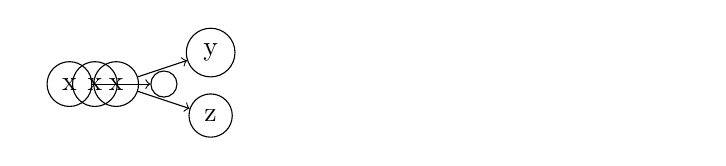
\begin{tikzpicture}
                \graphbox{$L$}{0mm}{0mm}{30mm}{20mm}{0}{0}{
                    \node[draw,circle]  (x) at (-6mm,-12mm) {x};
                    \node[draw,circle] (y) at (6mm,-12mm) {};
                    % \node[draw,circle]  (z) at (6mm,0mm) {};
                    \draw[->]  (x) to (y);
                    % \draw[->] (y) to[bend right=20] (z);
                    % \draw[->]  (z) to[bend right=20] (y);
                }
                \graphbox{$K$}{40mm}{0mm}{30mm}{20mm}{0}{0}{
                    \node[draw,circle]  (x) at (-6mm,-12mm) {x};
                    % \node[draw,circle]  (y) at (6mm,-12mm) {y};
                }
                \graphbox{$R$}{80mm}{0mm}{30mm}{20mm}{0}{0}{
                    \node[draw,circle]  (x) at (-6mm,-12mm) {x};
                        \node[draw,circle]  (y) at (6mm,-8mm) {y};
                        \node[draw,circle]  (z) at (6mm,-16mm) {z};
                        \draw[->]  (x) to (y);
                        \draw[->]  (x) to (z);
                }
                \node () at (35mm,-12mm) {$\leftarrowtail$};
                \node () at (75mm,-12mm) {$\rightarrowtail$};
            \end{tikzpicture}
        }
    \end{center}
    The set \( D(R,X) \) contains exactly two elements $R'$:
    \raisebox{2pt}{ 
        \scalebox{0.6}{\tikz[baseline=-0.5ex]{
        \node [draw,circle] (x) at (0,0) {x};
        \node[draw,circle] (y) at (1,0) {y};
        \draw[->] (x) -- (y) {};
    }}} and $R''$:\raisebox{2pt}{ 
        \scalebox{0.6}{\tikz[baseline=-0.5ex]{
        \node [draw,circle] (x) at (0,0) {x};
        \node[draw,circle] (y) at (1,0) {z};
        \draw[->] (x) -- (y) {};
    }}}. 
    Despite unique monomorphisms \( h_{R'L}: R' \rightarrowtail L \) and \( h_{R''L}: R'' \rightarrowtail L \) preserving interface elements, they fail the third condition of \autoref{def:creates_more_x_on_the_left}. 
    For any rewriting step using this rule, implicitly created $X$-occurrences with the same subgraph of the context have the same corresponding $X$-occurrence. 
\end{example}
 
\begin{example}
    \label{ex:cond4_necessaire}
    Let $X$ be the graph 
    \tikz[baseline=-0.5ex]{ 
            \node (x) at (0,0) {$\bullet$}; 
            \node (y) at (1,0) {$\bullet$};
            \node (z) at (2,0) {$\bullet$};
            \draw[->] (x) -- (y)   {};
    }, which has an isolated node. The following rewriting rule is potentially $X$-increasing.
    \begin{center}
        \resizebox{0.6\textwidth}{!}{
            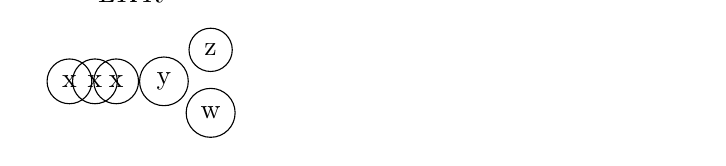
\begin{tikzpicture}
                \graphbox{$L$}{0mm}{0mm}{30mm}{20mm}{0}{0}{
                    \node[draw,circle]  (x) at (-6mm,-10mm) {x};
                    \node[draw,circle] (y) at (6mm,-10mm) {y};
                }
                \graphbox{$K$}{40mm}{0mm}{30mm}{20mm}{0}{0}{
                    \node[draw,circle]  (x) at (-6mm,-10mm) {x};
                }
                \graphbox{$R$}{80mm}{0mm}{30mm}{20mm}{0}{0}{
                    \node[draw,circle]  (x) at (-6mm,-10mm) {x};
                        \node[draw,circle]  (y) at (6mm,-6mm) {z};
                        \node[draw,circle]  (z) at (6mm,-14mm) {w};
                }
                \node () at (35mm,-10mm) {$\leftarrowtail$};
                \node () at (75mm,-10mm) {$\rightarrowtail$};
            \end{tikzpicture}
        }
    \end{center}
    The set \( D(R,X) \) contains exactly two elements $R'$:
    \raisebox{2pt}{\scalebox{0.6}{\tikz[baseline=-0.5ex]{
        \node [draw,circle] (x) at (0,0) {x};
        \node[draw,circle] (y) at (1,0) {z};
        % \draw[->] (x) -- (y) {};
    }}} and $R''$:\raisebox{2pt}{\scalebox{0.6}{\tikz[baseline=-0.5ex]{
        \node [draw,circle] (x) at (0,0) {x};
        \node[draw,circle] (y) at (1,0) {w};
        % \draw[->] (x) -- (y) {};
    }}}. 
    There are unique monomorphisms $h_{R'L}:R' \rightarrowtail L$ and $h_{R''L}:R'' \rightarrowtail L$ preserving interface elements, but they fail the fourth condition of \autoref{def:creates_more_x_on_the_left}.
    For any rewriting step using this rule, implicitly created $X$-occurrences with the same subgraph of the context have the same corresponding $X$-occurrence.
\end{example}